The future work will be focused on trying to find an answer to RQ3 during the second part of the research.
In order to achieve it, a detailed study of the current state of multi-robot choreography regarding emergent properties and collaborative adaptation must be performed.
%Nevertheless, since our plan is to continuously integrate all the obtained knowledge into the project, the framework developed during the first division of the project will be used and tested through this part as well.
%Furthermore, due to the tools created for the robot orchestration will be tested on real robots we still will need to deploy the software platform and its functionalities on each of them.
An architectural overview of the whole research is depicted in Figure~\ref{fig:overview}.
In this figure the expected final system is represented in a schematic way.
The aforementioned conceptual and temporal division of the research is expressed with dot-lined boxes.
The contents of the box concerning RQ1 comprehend everything since it represents a broad study.
%Then, the research concerning RQ2 is more focused.
The box that represents RQ2 contains a conceptual representation of a robotic team represented by a group of folded boxes that in turn contain the framework intended for each robot.
The communication methodology is also represented.
Then, the techniques that we plan to study in order to perform the choreography are contained in the RQ3 box.
%Note that the contents regarding RQ2 are embedded into RQ3.

During the second part of this PhD project, techniques for supporting the correct choreography of multiple robots will be studied and applied.
Robots should collaborate in a team to accomplish complex missions because often adaptations performed by a single robot are not sufficient to accomplish a specified mission. 
Tasks may need to be reassigned to other robots, or a team of robots needs to be reconfigured. 
Collaboration and interaction of robots among themselves and with the environment could lead to emergent properties representing unexpected behaviors. Emergent properties can be beneficial, neutral, or even harmful ---for instance, when they hamper safety or the mission accomplishment.

\begin{figure}[!t]
\begin{center}
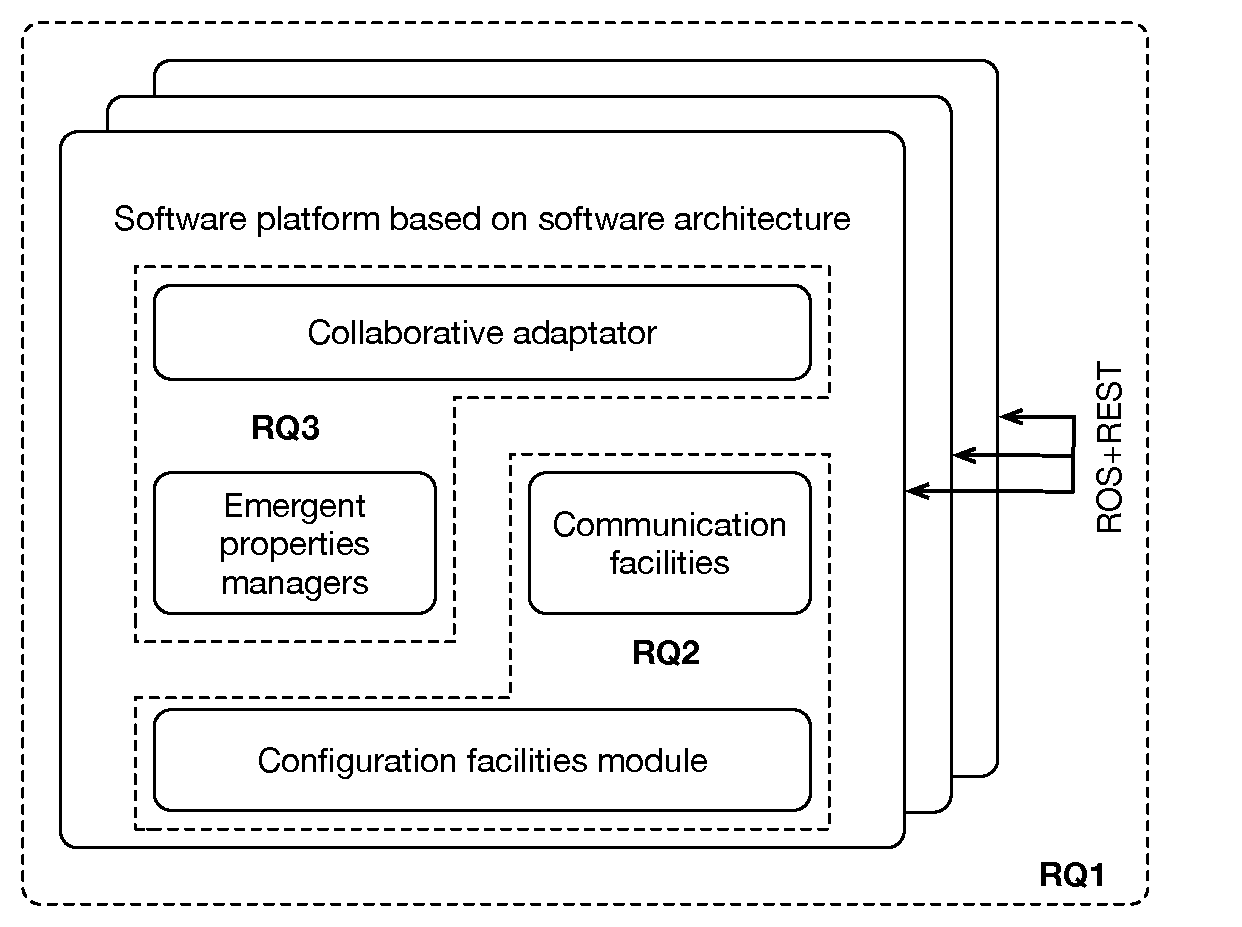
\includegraphics[width=1\linewidth]{Figures/research.pdf}
\caption{Architectural overview of the final system.}
\label{fig:overview}
\end{center}
\end{figure}